\documentclass{sigchi}


\usepackage{graphicx}    % This package is used for Figures
\usepackage{balance} % to better equalize the last page
\usepackage{times}    % comment if you want LaTeX's default font
\usepackage{url}      % llt: nicely formatted URLs
\usepackage{rotating}

% llt: Define a global style for URLs, rather that the default one
\makeatletter
\def\url@leostyle{%
\@ifundefined{selectfont}{\def\UrlFont{\sf}}{\def\UrlFont{\small\bf\ttfamily}}}
\makeatother
\urlstyle{leo}
% To make various LaTeX processors do the right thing with page size.
\def\pprw{8.5in}
\def\pprh{11in}
\special{papersize=\pprw,\pprh}
\setlength{\paperwidth}{\pprw}
\setlength{\paperheight}{\pprh}
\setlength{\pdfpagewidth}{\pprw}
\setlength{\pdfpageheight}{\pprh}

% Make sure hyperref comes last of your loaded packages, 
% to give it a fighting chance of not being over-written, 
% since its job is to redefine many LaTeX commands.
\usepackage[pdftex]{hyperref}
\hypersetup{
pdftitle={SIGCHI Conference Proceedings Format},
pdfauthor={LaTeX},
pdfkeywords={SIGCHI, proceedings, archival format},
bookmarksnumbered,
pdfstartview={FitH},
colorlinks,
citecolor=black,
filecolor=black,
linkcolor=black,
urlcolor=black,
breaklinks=true,
}

% create a shortcut to typeset table headings
\newcommand\tabhead[1]{\small\textbf{#1}}


\begin{document}

\title{Community Engagement and Response to First Time Code Contributors on 
GitHub}

\numberofauthors{2}
\author{
  \alignauthor 1st Author Name\\
    \affaddr{Affiliation}\\
    \affaddr{Address}\\
    \email{e-mail address}\\
    \affaddr{Optional phone number}
  \alignauthor 2nd Author Name\\
    \affaddr{Affiliation}\\
    \affaddr{Address}\\
    \email{e-mail address}\\
    \affaddr{Optional phone number}    
}

\maketitle                % create title and copyright pages

\keywords{
	open source; online communities; software development
}

\category{K.6.3.}{Management of Computing and Information Systems}{Software 
Management}

%%% Abstract %%%
\begin{abstract}           % abstract environment, this is optional
Using data from 13,383 first-time code contributions in 45 projects on GitHub, 
we analyzed whether social interactions impacted the acceptance of material 
contributions to FLOSS projects. We studied the behavior of developers before 
submitting code as well as community response to code contributions. We used 
comments on pull requests, comments on issues, and issue submissions as our 
primary measures of social interaction. We found that, for the most part, 
developers do not engage with the community on GitHub before submitting code 
changes. We also found that most code submissions do not elicit much community 
response. Social interaction by developers did have small positive effects on 
whether their code contributions were accepted, but the metrics we used for 
community response could not predict whether or not a pull request was 
accepted. Our findings suggest that, contrary to prior research in FLOSS and 
communities of practice, participation in social aspects of a project are not 
necessary for its success.
\end{abstract}

\section{Introduction}

As Free/Libre and Open Source Software (FLOSS) continues to grow and more users
become reliant on open source technologies, it is important to understand how
this software is developed. Research of open source software can also contribute
to existing research in a variety of other fields, including software
engineering and CSCW. Recruiting and retaining project contributors is crucial
to the success of open source projects, and this study examines the
relationships among community engagement, community response, and whether or not
code contributions are accepted. Much of the existing FLOSS research that
focuses on individual developers discusses motivations for
contributing~\cite{hann_economic_2002, krishnamurthy_intrinsic_2006}. We,
instead, focus on what happens immediately before and after an individual
actually contributes. Early success is a strong indicator of future engagement,
and our study helps us understand how a developer's social interactions and a
community's response influence whether a developer will experience early
success. As von Krogh points out, much of the work of socialization falls to the
newcomer~\cite{von_krogh_community_2003}, and we examine the social work
newcomers do in order to understand how their behavior influences whether or not
their material contributions will be accepted.

Specifically, we examine the behavior of first time code contributors and the
community response to their code contributions. We focus on code contributions
because they mark the first time a user is attempting to participate in a core
act of development. Code contributions can also be accepted or rejected, so our
analysis allows us to see how social factors contribute to acceptance within the
community. We provide evidence that the level of community engagement and
response a user gives and receives does not influence whether his/her code
contributions will be accepted. This finding indicates that FLOSS projects may
not actually need to foster community engagement or emphasize social processes
in order to succeed.

We studied projects hosted on GitHub, a social website that open source software
developers use to host their software projects and to browse other developers'
projects. It includes many features that are present on social networking sites,
such as the ability to follow other users and leave comments on projects. GitHub
provides a wealth of data for studying computer supported cooperative work, as
it is a centralized location where many different tasks take place. For example,
users can create bug reports, submit fixes, and engage in discussions about new
features all in one place.

The rest of this paper is organized as follows. First, we provide an overview of
GitHub terminology and a literature review on FLOSS and socialization. We then
describe our data collection and analysis methods. The discussion of our results
and how they differ from previous research in this area follow. We finish by
situating our findings in relation to prior research and identifying areas for
future work.


\subsection{Terminology} \label{sec:terms}

A software project on the website is referred to as a \textit{repository}. Any
user on GitHub can \textit{star} a repository. Users star repositories to be
able to easily navigate to them and to receive updates on activity from the
repositories. A repository can be private, meaning that it is only visible to
the owner and anyone the owner grants access to, or public, meaning that anyone
can view it. Our study focuses on public repositories. Many repositories use
\textit{issues} to organize workflow around bugs, features, enhancements, and
other code developments. Issues can be labeled, assigned to developers, and
associated with milestones. They can also be commented on and connected with
commits (e.g., associated with the commit that fixes a bug). Issues are also
marked `open' or `closed'. If a developer wants to contribute to another one of
developer's repositories, he can \textit{fork} the repository, which creates a
copy of the project for him to work on. As the developer makes changes to this
code, he \textit{commits} his changes. A \textit{commit} is a snapshot of the
code at a certain point in time. When the developer is finished, he can submit a
\textit{pull request} to the owner of the project. All pull requests for a
project are viewable on GitHub, and any user of the site can comment on them. A
pull request can have a status of open or closed. A status of open indicates
that that owner of the repository has not made a decision about whether or not
to include the changes. If the owner of a repository wants to incorporate the
changes the developer made, he can \textit{merge} them into the repository. A
pull request can be closed without being merged, which means that the changes
the developer made were not accepted.

\section{Related Work} \label{sec:relatedwork}

\subsection{FLOSS Research} Research in the development of FLOSS has grown
tremendously in the last several years. Crowston et
al.~\cite{crowston_free/libre_2008} note the importance of understanding FLOSS
development as it becomes a major social movement with many volunteers
contributing to projects and many FLOSS projects becoming integral parts of the
infrastructure of modern society (e.g., Apache, Python). Other researchers have
emphasized the role that FLOSS research can play in improving current existing
research of software engineering, particularly as the importance of
understanding large scale software systems in science and industry increases
~\cite{scacchi_free/open_2007}.

Existing research approaches FLOSS from many different angles, including
motivation of open source developers~\cite{fang_understanding_2009,
lakhani_why_2003, shah_motivation_2006}; governance of
FLOSS~\cite{hippel_open_2003, omahony_guarding_2003, omahony_governance_2007};
and knowledge sharing within FLOSS communities~\cite{endres_tacit_2007,
hemetsberger_collective_2009, sowe_understanding_2008}. Our study focuses on the
behavior of first-time contributors to FLOSS projects and how the community
responds to their contributions. We build on previous studies that describe the
social processes of community joining~\cite{ducheneaut_socialization_2005,
huang_mining_2005, von_krogh_community_2003}. Given the distributed nature of
FLOSS development, our findings potentially contribute to our understanding of
virtual work and distributed teams more broadly as well.

GitHub is a relatively new social FLOSS platform and has not been extensively
studied. CSCW researchers provide some notable exceptions, however. Dabbish et
al.~\cite{dabbish_social_2012} found that the transparency GitHub provides leads
to inferences around commitment, work quality, community significance and
personal relevance, which supports collaboration and learning. McDonald and
Goggins~\cite{mcdonald_performance_2013} studied how different communities on
GitHub measure success and found that most developers measure success in the
number of contributors and contributor growth. They also found that developers
believed the GitHub interface, in particular the use of pull requests, made
communities more democratic and transparent. Choi et
al.~\cite{choi_herding_2013} leveraged data from a sample of GitHub projects to
contribute to theories of developer coordination, finding that commits tend to
happen in clustered events over time. In all these cases, the social features of
GitHub, e.g. the ability to follow other users and view information about them,
provide new ways to study social behavior in FLOSS projects. Our study
investigates members' participation in group discussions on the site. While
previous studies have tried to combine data from mailing lists and version
control~\cite{ducheneaut_socialization_2005}, GitHub provides a centralized
location to study communities in which discussions and code contributions occur
in one place. At least with regards to user support, recent research suggests
that developers may be moving away from mailing lists to social Q\&A sites to
respond to user requests for help~\cite{vasilescu_how_2014}. By focusing on
GitHub data, we contribute to understanding developer behavior on this new
social platform.

\subsection{Socialization and Joining Professional Communities}
\label{sec:communities} Our study focuses on the behavior of new code
contributors and community response to their contributions. We use the
theoretical framework of \textit{legitimate peripheral participation} (LPP)
~\cite{lave_situated_1991} in our exploration community joining. LPP describes a
process of learning in communities of practice in which newcomers join a
community by participating in peripheral tasks and forming relationships to move
towards the center of the community. LPP and communities of practice are also
often leveraged in other studies of computer mediated communication. For
example, Bryant and colleagues ~\cite{bryant_becoming_2005} note that members of
Wikipedia initially become involved through peripheral activities -- simple and
low risk activities members can take part in to learn more about the community
before trying to become major contributors.

Several studies of FLOSS development have used the LPP framework, e.g., to
identify core and peripheral community members~\cite{huang_mining_2005}, to
understand motivation in FLOSS communities~\cite{ye_toward_2003}, and to develop
the concept of a \textit{joining script}~\cite{von_krogh_community_2003}. A
\textit{joining script} is a set of tasks for new developers to go through
before being accepted into the community~\cite{von_krogh_community_2003}.
Similarly, Ducheneaut~\cite{ducheneaut_socialization_2005} found a pattern that
resembles LPP in his study of contributors to the Python project.

GitHub's tools (e.g., issues) enable potential developers to observe both the
code and social conventions of a community before joining. Those tools also
enable us to collect data to examine a number of legitimate peripheral
activities in FLOSS development. For instance, opening and commenting on issues,
submitting and commenting on pull requests are all low risk activities new
developers can engaged in via GitHub. Existing members can also provide feedback
about issues, comments, and code submitted through the site. Prior research
relied on version control histories~\cite{huang_mining_2005} and/or mailing list
data~ \cite{ducheneaut_socialization_2005, von_krogh_community_2003} to
understand social and development activities, and using GitHub data allows us to
explicitly connect social and code contributions and to examine their
relationships.

In this study, we focus on behavior leading up to a developer's first pull
request.  Previous studies have distinguished types of activity in FLOSS
repositories and found there is a core group of developers who work on
functionality while most members of the community contribute through
participating in activities such as reporting bugs and technical
discussions~\cite{dinh2005freebsd, mockus2002two}. Previous studies have also
shown that developers who contribute code to the repository go through a
socialization phase by participating in these peripheral activities and then
moving towards the central group of primary
developers~\cite{ducheneaut_socialization_2005, von_krogh_community_2003}. We
study activity prior to the first pull request to understand this socialization
process and how it affects community response to code contributions.

Our study examines community response to a user's first pull request. Research
on Wikipedia has shown that community response to newcomers' contributions
affects their long term commitment to the project~\cite{choi2010socialization}.
We expect a similar effect in FLOSS projects. Shibuya and
Tamai~\cite{shibuya2009understanding} found that at least one factor that
contributes to difficulty for newcomers to FLOSS projects is a lack of response
from core developers. We focus on response to a user's first pull request as
this represents a critical moment in the socialization process of newcomers.

\section{Methods} \label{chap:methods}

\subsection{Data Collection} \label{sec:datacollection}

Data was collected using the GitHub API.\footnote{http://developer.github.com/}
We used a collection of node.js scripts to collect data from the API to store in
a MySQL database.\footnote{These scripts are available at [Removed for blind
review].} In selecting which repositories to use for our analysis, we started
with the top 100 most starred repositories on GitHub. We started with this list
with the assumption that they were popular repositories that would be maintained
by an active community. From these 100, we manually filtered out certain
projects that we expected would follow different development patterns than a
typical programming project, for example, collections of configuration files for
text editors and shells, collections of icons, etc. We also excluded
repositories that were used primarily for demonstration or documentation
purposes, such as sample web applications to demonstrate use of a certain web
framework. After filtering our intial list of 100, 45 repositories remained in
our data set for analysis. We consider only pull requests with a status of
closed. This resulted in approximately 44,400 pull requests. We further filtered
this data by selecting only the first pull request a user submitted to a
repository, leaving 13,383 pull requests. The distribution of these pull
requests across repositories ranges from 10 to 1,489, with a median of 210. To
find merged pull requests, we first filter all pull requests that are marked as
merged by the GitHub API, meaning that the project maintainers used GitHub's
merge feature to accept the pull request. In some repositories, project
maintainers use a different workflow when accepting pull requests, wherein the
code changes are accepted, but it is not reflected as merged on GitHub. In most
of these cases, there is a standard way of reflecting this in the commit
comments, so we use some naive heuristics for identifying these requests by
searching commit comments for certain text patterns. For example, in many
projects, the project maintainer will manually add the commits from the pull
request, and create a new commit with a commit message that follows the pattern
"Closes {number}" where {number} is the pull request ID on GitHub. Finding
merged pull requests using both the status from the GitHub API as well as these
text patterns results in finding 5,239, or 39.1\% of first pull requests being
merged.

\subsection{Data Analysis} \label{sec:data_analysis} We primarily used logistic
regression for our statistical analysis. In all cases, we use various aspects of
developer engagement and community response to predict whether or not a pull
request is merged. We also included controls for the changes and contributors in
a repository, but those controls never produced an improvement in the models.
Below we discuss the predictors we used.

\subsection{Developer's Engagement} To measure developer engagement, we use four
variables: the number of pull requests s/he commented on, the number of issues
s/he commented on, the number of issues s/he submitted, and his/her reputation.
Not all repositories in our data set use GitHub issues, so for those
repositories, we only consider the number of previous pull requests a developer
commented on. Previous studies indicate that users participate in technical
discussions before submitting code~\cite{von_krogh_community_2003}.
Figure~\ref{fig:up} plots the sum of the interaction variables (excluding
reputation) by the number of repo.

\begin{figure*}[p] \centering
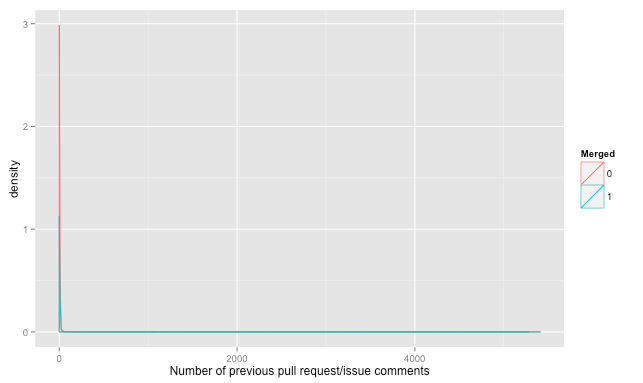
\includegraphics[width=0.8\textwidth]{figures/number_comments_density_ggplot.png}
\caption{User participation density plots.} \label{fig:up} \end{figure*}

\begin{figure*}[p] \centering
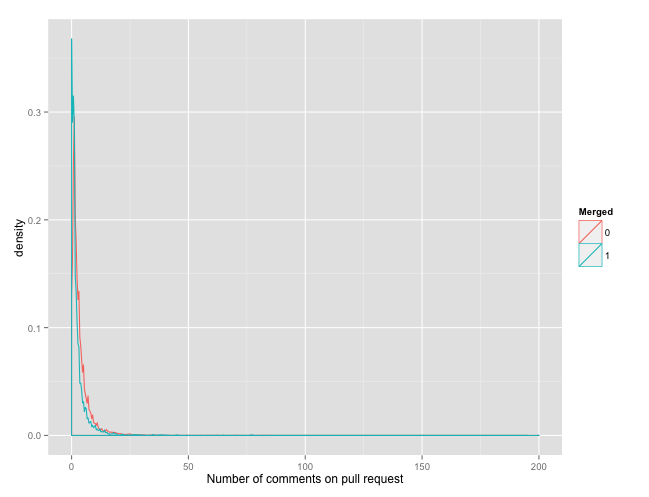
\includegraphics[width=0.8\textwidth]{figures/comments_on_pr_density_ggplot.png}
\caption{Attention pull request receives density plots.} \label{fig:aprr}
\end{figure*}

\subsection{Community's Response} In addition to measuring the activity of a
developer in the community before submitting a pull request, we are also
interested in measuring the community response to a given pull request and how
that response relates to whether or not a pull request is accepted. We measure
this in two ways.

First, we simply count the number of comments on a given pull request. This is
used as a basic metric of how much attention a pull request receives. This
variable is shown in Figure~\ref{fig:aprr}.

Our next analysis of community response focuses on the language of the comments
on a pull request. To test whether or not the content of these comments is
predictive of whether or not a pull request is merged, we collect the comments
for each of our first pull requests. We ignore comments made by the user who
submitted the pull request, since we are interested in what other users had to
say about it. We also ignore the last comment associated with a pull request,
since these often will explicitly say whether or not the maintainer is merging
the pull request or not. We are interested in whether the type of language used
in the discussion of a pull request is predictive of whether or not it is
accepted. We ignore pull requests that only have one comment associated with it.
This leaves 5,674 pull requests. Of these, 3,811, approximately 67\%, were not
accepted. We treat the remaining comments associated with the pull request as
one document, and convert them into feature vectors representing the count of
each unigram and bigram in the documents, after using a word list to remove stop
words. We then train both a logistic regression and naive Bayes classifier using
this feature set. The results of testing these classifiers is shown in
Table~\ref{tbl:classifiers}. The results shown are the result of running 10-fold
cross validation.

\begin{table}[ht] \centering
  \caption{Classifier results}
  \label{tbl:classifiers}
  \begin{tabular}{lll}
  \hline\hline
  ~         & Logistic Regression & Naive Bayes \\
  Accuracy  & 69.6\%              & 70.4\%      \\
  Precision & 56.3\%              & 56.3\%      \\
  Recall    & 33.7\%              & 44.4\%      \\
  \hline
  \end{tabular}
\end{table}

\newpage
\section{Results} \label{chap:results}
Tables~\ref{tbl:logit_coef} and \ref{tbl:logit_odds} summarize the results of our logistic regressions 
using developer and community behaviors to predict whether pull requests are 
merged. Overall, we found that participating in technical discussions through 
pull request comments and issue comments made statistically significant 
difference on whether or not a pull request was merged, but the difference was 
so small as to be practically meaningless. Table~\ref{tbl:logit_coef} shows the 
results of the logistic regressions and displays the coefficients and standard 
errors for each predictor. Table~\ref{tbl:logit_odds} shows the same models but 
provides odds ratios and confidence intervals instead. We discuss the results 
of these regressions in detail and provide additional descriptive statistics below.

\begin{table}[!htbp] \centering 
  \caption{Descriptive statistics for predictors included in logistic regressions} 
  \label{tbl:descriptives} 
\begin{tabular}{@{\extracolsep{5pt}}lrrrr} 
\\[-1.8ex]\hline 
\hline \\[-1.8ex] 
 & \multicolumn{2}{c}{Merged} & \multicolumn{2}{c}{Not Merged} \\ 
Statistic & \multicolumn{1}{c}{Mean} & \multicolumn{1}{c}{St. Dev.} & 
\multicolumn{1}{c}{Mean} & \multicolumn{1}{c}{St.Dev} \\ 
\hline \\[-1.8ex] 
\multicolumn{5}{l}{Developer Variables} \\
Reputation & 129.92 & 949.68 & 83.08 & 513.08  \\  
PR comments & 0.78 & 15.44 & 0.25 & 3.28\\ 
Issue comments & 3.71 & 66.77 & 1.69 & 22.77  \\ 
Issues opened & 0.68 & 5.25 & 0.48 & 2.28 \\ 
\multicolumn{5}{l}{Community Variables} \\
PR comments & 2.73 & 5.64 & 3.25 & 4.43 \\ 
\hline \\[-1.8ex] 
\end{tabular} 
\end{table}

Our descriptive statistics (Table~\ref{tbl:descriptives}) show remarkable 
variation in all measures of engagement. All of the means are quie low, though 
issue comments and pull request comments posted by community members are 
slightly more common than other types of engagement.

\begin{table*}[!htbp] \centering 
  \caption{Logisitic regressions: Predicting pull request merges (coefficients)} 
  \label{tbl:logit_coef} 
\begin{tabular}{@{\extracolsep{5pt}}lcccccc} 
\\[-1.8ex]\hline  
\\[-1.8ex] & (1) & (2) & (3) & (4) & (5) & (6)\\ 
\hline \\[-1.8ex] 
 Reputation &  & 0.0001$^{***}$ & 0.0001$^{***}$ &  & 0.0001$^{***}$ & 0.0001$^{**}$ \\ 
  &  & (0.00003) & (0.00003) &  & (0.00003) & (0.00003) \\ 
  & & & & & & \\ 
 Pull request comments (developer) & 0.014$^{***}$ & 0.010$^{**}$ & 0.011$^{***}$ &  &  & 0.014$^{**}$ \\ 
  & (0.005) & (0.005) & (0.004) &  &  & (0.006) \\ 
  & & & & & & \\ 
 Issue comments &  &  &  & 0.001 & 0.001 & $-$0.001 \\ 
  &  &  &  & (0.001) & (0.001) & (0.001) \\ 
  & & & & & & \\ 
 Issues opened &  &  &  & 0.016$^{*}$ & 0.016$^{*}$ & 0.016$^{**}$ \\ 
  &  &  &  & (0.008) & (0.008) & (0.008) \\ 
  & & & & & & \\ 
 Pull request comments (others) &  &  & $-$0.030$^{***}$ &  &  & $-$0.030$^{***}$ \\ 
   &  &  & (0.004) &  &  & (0.004) \\ 
   & & & & & & \\
 Constant & $-$0.446$^{***}$ & $-$0.453$^{***}$ & $-$0.364$^{***}$ & $-$0.453$^{***}$ & $-$0.459$^{***}$ & $-$0.372$^{***}$ \\ 
  & (0.018) & (0.018) & (0.022) & (0.018) & (0.018) & (0.022) \\ 
  & & & & & & \\ 
\hline \\[-1.8ex]  
\multicolumn{7}{l}{\textit{Note:} $^{*}$p$<$0.1; $^{**}$p$<$0.05; $^{***}$p$<$0.01} \\ 
\end{tabular} 
\end{table*}

\begin{table*}[!htbp] \centering 
  \caption{Logisitic regressions: Predicting pull request merges (odds ratio and confidence intervals)} 
  \label{tbl:logit_odds} 
\begin{tabular}{@{\extracolsep{5pt}}lcccccc} 
\\[-1.8ex]\hline 
\hline \\[-1.8ex] 
\\[-1.8ex] & (1) & (2) & (3) & (4) & (5) & (6)\\ 
\hline \\[-1.8ex] 
 Reputation &  & 1.00 & 1.00 &  & 1.00 & 1.00 \\ 
  &  & (1.00, 1.00) & (1.00, 1.00) &  & (1.00, 1.00) & (1.00, 1.00) \\ 
  & & & & & & \\
 PR comments (developer) & 1.01 & 1.01 & 1.01 &  &  & 1.01 \\ 
  & (1.01, 1.03) & (1.00, 1.02) & (1.01, 1.02) &  &  & (1.00, 1.03) \\ 
  & & & & & & \\ 
 Issue comments &  &  &  & 1.00 & 1.00 & 1.00 \\ 
  &  &  &  & (1.00, 1.00) & (1.00, 1.00) & (1.00, 1.00) \\ 
  & & & & & & \\ 
 Issues opened &  &  &  & 1.02 & 1.02 & 1.02 \\ 
  &  &  &  & (1.00, 1.03) & (1.00, 1.03) & (1.00, 1.03) \\ 
  & & & & & & \\ 
  PR comments (others) &  &  & 0.97 &  &  & 0.97 \\ 
   &  &  & (0.96, 0.98) &  &  & (0.96, 0.98) \\ 
   & & & & & & \\
 Constant & 0.64 & 0.64 & 0.69 & 0.64 & 0.63 & 0.69 \\ 
  & (0.62, 0.66) & (0.61, 0.66) & (0.67, 0.73) & (0.61, 0.66) & (0.61, 0.66) & (0.66, 0.72) \\ 
  & & & & & & \\ 
\hline \\[-1.8ex] 

\multicolumn{7}{l}{\textit{Note:} $^{*}$p$<$0.1; $^{**}$p$<$0.05; $^{***}$p$<$0.01} \\ 
\end{tabular} 
\end{table*}

\subsection{Developer's Engagement} \label{results_engagement}

\subsubsection{Pull Requests}

We see that user participation for the majority of all first pull requests, both
merged and not merged, is 0. This indicates that in general, most users are not
attempting to engage in the peripheral activity of commenting on other pull
requests before submitting their own. The GitHub interface makes it relatively
easy for a user to fork a repository, make changes, and submit the changes for
consideration. Previous studies on GitHub have shown that the number of
contributions did increase for some projects that moved from other hosting
options to GitHub~\cite{mcdonald_performance_2013}. It is possible this
interface lowers the barrier of entry for a developer who wants to contribute to
a project, and allows them to bypass participating in the joining script
described by von Krogh et al. ~\cite{von_krogh_community_2003}.

We also examine these variables for first pull requests by users who later
submit another pull request. We want to see whether or not this ``no engagement"
pattern continues to hold for users who will become active contributors. Our
intuition here is that some users might encounter a bug they fix or desire a
feature that they implement, and then submit these changes back to repository.
They may not comment on other pull requests as they are not interested in
becoming long term members of the community, but rather are just interested in
submitting a one time patch. Users who do plan on becoming active members,
however, may participate in peripheral activities more.
Figure~\ref{fig:repeaters} shows a visualization of the same first pull
requests, but only for users who submit at least one other pull request at a
later point in our data set, and Figure~\ref{fig:repeaters_10} shows the data
for users who submit at least 5 more times. Looking at users who submit at least
one other time cuts our number of observations from 13,383 to 5,207, indicating
that approximately 61\% of these pull requests come from users who will not
contribute any others. Looking at users who will submit at least 10 more times
gives us a total of 1,155 observations.

It is clear that in all these cases, regardless of whether or not they will be
continuing to submit other pull requests later, at the time of submitting their
first pull request, users are generally \textit{not} participating socially in
the community. The previous graphs only consider the number of pull requests a
user commented on before submitting their first pull request, so we do not
capture how users who submit multiple pull request over time comment on other
pull requests over time. In Figure~\ref{fig:commented_pullrequests_totals} we
plot the total number of others' pull requests that a user commented on by how
many pull requests they submitted themselves, considering only users who have
submitted at least two pull requests. There is not a strong correlation between
these variables (Spearman's $\rho$ = 0.44), indicating that users do not
necessarily participate in more commenting as they continue to submit more pull
requests.

The results of our logistic regressions suggest that developers who comment on 
pull requests before submitting their own are slightly more likely to have 
their own pull request merged (see Models 1-3 and 6 in 
Table~\ref{tbl:logit_coef}). Though the effect is statisticall significant, the 
odds ratio and confidence interval show that the effect is quite small (OR = 
1.01). This effect holds when we control for developer's 
reputation and community's response as well. 

It's worth noting the one extreme outlier present in our data. One
user-submitted pull request received 200 comments and was submitted by a user
who had commented on 900 previous pull requests. This is an interesting case of
a project maintainer, who has commit access and wouldn't typically need to
submit a pull request to submit changes, creating a pull request for commits
related to a major upgrade in the project. By creating a pull request, he was
able to document all the changes associated with this change and allow community
members to ask questions or comment on the changes. He has a high number of
previous comments since he is in charge of accepting pull requests and often
posts a comment such as, ``Accepted" when accepting a pull request. This outlier
likely received so many comments because many other developers were asking
questions or voicing their opinions. This example demonstrates the different
ways pull requests may be used in different projects, and how the way they are
used may change depending on the type of user submitting them.

\begin{figure*}[p] \centering
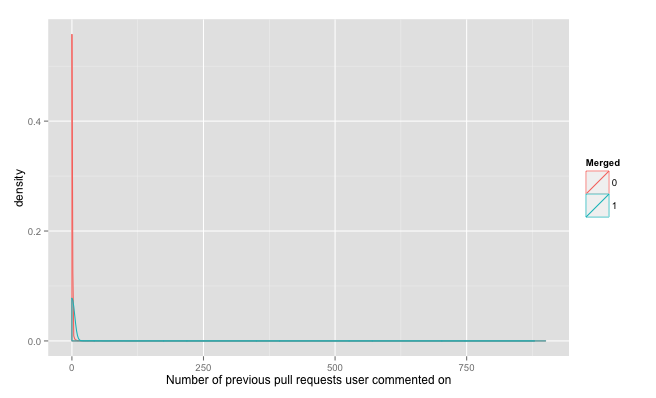
\includegraphics[width=0.8\textwidth]{figures/number_comments_density_repeaters_ggplot.png}
\caption{User participation density plots for users who submit at least one
other pull request in our data set.} \label{fig:repeaters} \end{figure*}

\begin{figure*}[p] \centering
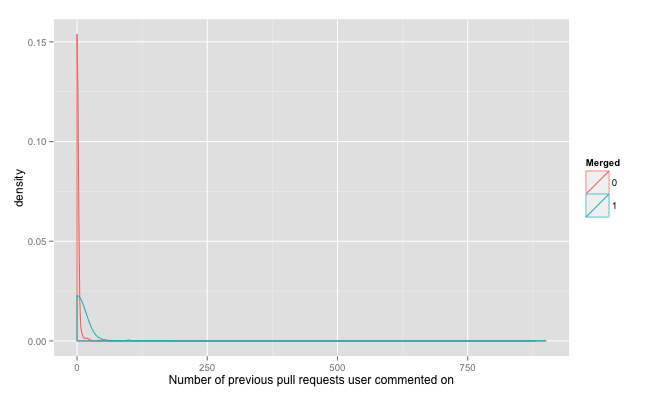
\includegraphics[width=0.8\textwidth]{figures/number_comments_density_repeaters_10_ggplot.png}
\caption{User participation density plots for users who submit at least ten
other pull requests in our data set.} \label{fig:repeaters_10} \end{figure*}

\begin{figure*}[htbp] \centering
\includegraphics[width=0.8\textwidth]{figures/commented_pullrequests_totals_ggplot.png}
\caption{Total number of pull requests commented on and total number of pull
requests submitted for each user.} \label{fig:commented_pullrequests_totals}
\end{figure*}

\subsubsection{Issues}

We also examined the effects of participating in discussions about issues and 
found that commenting on issues does not impact whether a developer's pull 
request will be merged (see Models 4-6 in 
Table~\ref{tbl:logit_coef}). Opening issues, however, has a small significant 
positive effect (OR = 1.02) on whether one's pull request will be merged. 
Though, 1.00 falls within the confidence interval for issues opened, so the 
statistical effect may actually be practically meaningless.

\subsection{Community's Response} 
In Figure~\ref{fig:up}, we see more variance
in the number of comments on first pull requests than we did with the number of
pull requests users commented on before submitting. However, this variable does
not seem to be a good predictor of whether or not a pull request is merged,
since both the merged and not merged distributions follow a similar pattern. It
seems just viewing the amount of activity a pull request receives is not enough
to explain whether or not it gets merged.

Training classifiers using the comment text may help address this problem, as
this can capture the valence of the comments, rather than just the raw number.
However, the low recall rates we see in Table~\ref{tbl:classifiers} indicate
that the text data is not sufficient to distinguish positive cases. We list the
top five features for each class in Table~\ref{tbl:features}. Despite leaving
out the last comment from each comment thread to avoid words that explicitly
describe the action being taken, we still see these in our top features. Both
"land" and "landed" are used in some repositories when a commit is merged, but
not through the GitHub interface to indicate the git commit hash where the pull
request commits were merged. We also see "closing" in the negative class, which
shows explicit action being taken. Some of the larger projects also skew our
results, as we see project names appear as the highest ranking features of the
negative class. Some of our top features do seem fitting. The phrase "lgtm"
which stands for "looks good to me" seems indicative of positive feedback from
the community.

Our sample size of 5,674 is relatively small, but it is interesting to note that
only 42\% of the first pull requests in our data set have more than 1 comment
associated with them. Our research question that drove these experiments was how
community response affects whether or not a pull request is accepted. However,
we see that the majority of pull requests don't attract any community attention.

\begin{table}[ht] \centering
\caption{Classifier top features}
\label{tbl:features}
\begin{tabular}{ll|ll}
\hline\hline
Merged  & ~     & Not merged  & ~      \\
land    & 0.981 & bootstrap & -0.780 \\
landed  & 0.894 & spree   & -0.875 \\
cla thanks    & 0.874 & closing & -0.641 \\
fine    & 0.721 &  already & -0.600 \\
lgtm    & 0.688 & maybe & -0.597 \\
\hline
\end{tabular}
\end{table}

\section{Discussion} \label{chap:conclusion}

In this study, we analyzed community engagement and community response of first
time code contributors on GitHub. We found that most developers do not engage by
participating in discussions on GitHub before submitting code changes. We also
found that most submitted pull requests do not attract much community response,
and our attempts at measuring community response did not provide good predictors
for whether or not a pull request is accepted. Our findings have implications
for researchers, open source contributors, and open source project maintainers.

We found that most users do not engage with the community in the way we expected
from previous FLOSS and LPP literature. Some reasons for this are discussed
below in Section~\ref{sec:future_work}. Since GitHub is a new platform that
encourages new types of social interactions, it can be used as a new source of
data to study open source communities. Our study focused on a relatively small
number of repositories pulled from the most starred repositories on GitHub.
Further work should be done on a larger sample of different types of
repositories. It's possible that new types of social websites like GitHub will
require new theoretical ways of thinking about distributed work and virtual
teams.

The majority of first pull requests in our data set were not accepted, but
community engagement is not a good predictor or whether or not they are
accepted, and most developers do not engage before submitting a pull request,
even if they end up becoming active code contributors. The implication for
developers who want to become involved in an open source project on GitHub is
that they do not necessarily need to participate in peripheral activities before
submitting pull requests. Although our study did not identify which factors do
contribute to acceptance of pull request, it's possible that developers should
focus more on things like finding relevant issues to fix or features to work on
rather than on social interactions.

Many open source projects fail due to insufficient volunteer
participation~\cite{crowston_defining_2003,krishnamurthy_cave_2002}. It
is therefore important for project maintainers to continue to attract volunteer
developers to keep a project alive. We found that 61\% of first pull requests in
our data set come from users who will not submit any other pull requests.
Project owners should consider ways to convert these one time contributers to
regular active contributors.

Our major finding in this study is that, despite previous FLOSS research which
did indicate social patterns that follow legitimate peripheral participation
framework~\cite{ducheneaut_socialization_2005, huang_mining_2005,
ye_toward_2003}, we generally do not see this pattern in our GitHub data set.
Although some developers do leave comments on other pull requests before
submitting their own, the majority of developers do not, including those that
will continue to submit code changes. Similarly, developers do not comment on 
or submit issues before submitting pull requests. When developers do engage in
social interaction before submitting a pull request, they gain only marginal
increases in the odds that their code will be accepted.

There are many reasons users do not socially interact before submitting 
material contributions to FLOSS projects on GitHub. As mentioned in 
Section~\ref{results_engagement}, GitHub's interface makes it
fairly easy to submit changes. Users only need to click a button to create a
copy of the repository that they can make commits on, and then click another
button to submit those commits as a pull request when they are finished. This
process may lower barriers to entry for new developers. While previous studies
of FLOSS communities have focused on mailing lists and centralized version
control repositories, the distributed nature of git may be altering the social
patterns that take place in developer networks. This study may suggest we need
to alter existing social theory as new interfaces change social interactions.

\subsection{Limitations} \label{sec:limitations}

This study only focused on data from GitHub, and our notion of community
engagement by developers was limited to activity by developers on GitHub. While
we have shown that this data is not sufficient to predict whether or not a pull
request is merged, further studies should create joint data sets merging GitHub
data with data from other sources, such as mailing lists, forums, or chat rooms
to test whether or not developers engage with the community using these other
platforms, and how those social interactions affect their acceptance in the
community. Though GitHub is designed to house all of a project's information,
many projects still use other channels for discussion that aren't included in
our data. One difficulty in creating these types of data sets is identify
merging, the process of matching different logins from different services to the
same physical person, but a number of techniques have been proposed to assist in
this process~\cite{bird_open_2007, goeminne_comparison_2013, kouters_whos_2012}.

It is also important to note that the GitHub platform is used in different ways
across projects. As described in Section~\ref{sec:datacollection}, there was
some work required to identify merged pull requests due to the different ways a
project maintainer accepts the pull request, e.g. through the GitHub interface
or not. In Section~\ref{results_engagement}, we discuss an outlier in our data
where a user who did not typically contribute code through the pull request
mechanism did use this feature in order to allow community feedback and
questions. There are many other examples of differences in use of the GitHub
platform. Some projects, for example, may require all developers to submit pull
requests for the purposes of code review, while others may grant commit access
to certain developers, allowing them to bypass the pull request mechanism
altogether. Although we did account for differences in accepting pull requests,
there may be other nuances across projects that affect the data we collected
that are harder to detect when working with data at scale.

\subsection{Future Work} \label{sec:future_work}

In examining developer engagement and community response, our study was
primarily concerned with social factors within FLOSS development
communities. It's possible that looking at only social factors is not enough to
understand what contributes to code acceptance on GitHub. Static analysis tools 
may be used in addition to the metrics we used in this study to further explore 
how the code itself affects whether or not a pull request is accepted.

In studying how communities respond to pull requests, we found in most cases,
there was little community response. As mentioned above, attraction of new
developers and retention of developers is important to project success. Future
work should explore how community response can affect developer retention in
GitHub projects.

In examining the top features for the classifiers we trained in studying
community response, we found some issues. Our goal in filtering the text
collected was to avoid words that explicitly described action being taken. We
still found examples of these types of words in both our positive and negative
classes. In the case of the positive (merged) class, the top feature was "land."
This feature affects classifier performance since this word is used often in
positive cases, but only in a few repositories. Similarly, project titles were
often predictive of acceptance but those terms are not useful for predicting
acceptance across projects. Future work studying linguistic features in this way
should account for these types of project-specific vocabularies.

Our analysis focused only on behavior of developers leading up to the submission
of their first pull request and the community response to that pull request. We
consider this a critical moment in the the socialization process since this task
is often considered as a core task that a developer can participate in. Future
studies should invetigate how community response at this moment affects
continued contribution and commitment to the project by developers.

Finally, to better understand the way that the GitHub interface affects
developer behavior will require further qualitative study. While there have been
surveys of GitHub developers previously~\cite{mcdonald_performance_2013}, there
remains a lot of work left to do in this area. The traces of behavior visible in
GitHub data tell us only part of the story.

\section{Conclusion}

In this study, we measured developer engagement and community response of first
time code contributors to GitHub and tried to predict whether code contributions
would be accepted based on that data. We found that most users do not
participate in social GitHub features before submitting code. In attempting to
measure community response, we found that most code contributions do not receive
much community response, and that both the raw amount of comments on a GitHub
pull request as well as the language in those comments were not good predictors
of whether or not the pull request is accepted. These findings suggest that
social interaction is not a necessary component of successful FLOSS projects.

\balance

%
% BIBLIOGRAPHY
%
\bibliographystyle{acm-sigchi}
\bibliography{Master}
\end{document}
